\documentclass[tikz,border=10pt]{standalone}
\usepackage{amsmath,amssymb,latexsym}
\usepackage{enumerate}
\usepackage{bm}
\usepackage{mathrsfs,marvosym,textcomp}
\usepackage{stmaryrd}
\usepackage{graphicx, subfigure}
\usepackage{color}
\usepackage[all]{xy}
\usepackage{extarrows}
\usepackage{proof}
\usepackage{hyperref}
\usepackage{wrapfig}
\usepackage{multirow}
\usepackage{epstopdf}

\begin{document}
    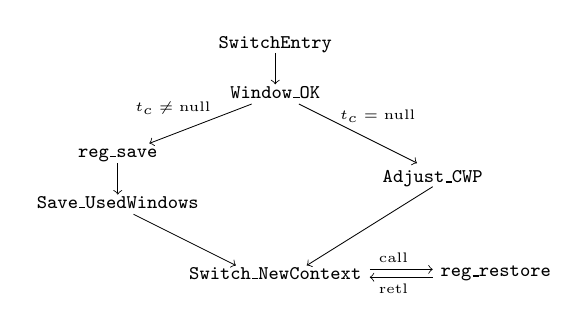
\begin{tikzpicture}[font=\scriptsize, line width=0.3pt]
        \node(SwitchEntry) at (0, 2) {\texttt{SwitchEntry}};
        \draw[->] (0, 1.9) -- (0, 1.5);

        \node(WindowOK) at (0, 1.4) {\texttt{Window\_OK}};
        \draw[->] (-0.3, 1.25) -- (-1.6, 0.75);
        \node(tcneqnull) at (-1.3, 1.2) {\tiny$t_c \neq \text{null}$};
        \draw[->] (0.3, 1.25) -- (1.8, 0.5);
        \node(tceqnull) at (1.3, 1.1) {\tiny$t_c = \text{null}$};

        \node(regsave) at (-2, 0.6) {\texttt{reg\_save}};
        \draw[->] (-2, 0.5) -- (-2, 0.1);
        \node(SaveUsedWindows) at (-2, 0) {\texttt{Save\_UsedWindows}};
        \draw[->] (-1.8, -0.15) -- (-0.5, -0.8);

        \node(AdjustCWP) at (2, 0.3) {\texttt{Adjust\_CWP}};
        \draw[->] (2, 0.2) -- (0.4, -0.8);
        \node(SwitchNewContext) at (0, -0.9) {\texttt{Switch\_NewContext}};

        \node(regrestore) at (2.8, -0.9) {\texttt{reg\_restore}};
        \node(call) at (1.5, -0.7) {\tiny\text{call}};
        \draw[->] (1.2, -0.85) -- (2, -0.85);
        \node(retl) at (1.5, -1.1) {\tiny\text{retl}};
        \draw[->] (2, -0.95) -- (1.2, -0.95);
    \end{tikzpicture}
\end{document}
